\documentclass[useAMS,usenatbib]{mn2e}
\usepackage{myaasmacros}
\usepackage{graphicx}
\usepackage{ulem}
\usepackage{amsmath}
\usepackage{multirow}

% Some definitions of things I always use here:
\def\ltsima{$\; \buildrel < \over \sim \;$}
\def\simlt{\lower.5ex\hbox{\ltsima}}   
\def\gtsima{$\; \buildrel > \over \sim \;$}
\def\simgt{\lower.5ex\hbox{\gtsima}}

%Code definition:
\def\Glass{{\sc Glass}}
\def\PixeLens{{\sc PixeLens}}

\title[Light versus Dark in Strong Lensing Galaxies]{Light versus Dark in Strong  Lensing Galaxies: Dark matter halos are rounder than their stars}

\author[Bruderer]{Claudio Bruderer$^{1}$\thanks{E-mail: claudio.bruderer@phys.ethz.ch}, J. I. Read$^{1,2}$, P. Saha$^{3}$, J. Coles$^{4}$\\
$^{1}$Institute for Astronomy, Department of Physics, ETH Z\"urich, Wolfgang-Pauli-Strasse 27, CH-8093 Z\"urich, Switzerland\\
$^{2}$Department of Physics, University of Surrey, Guildford, GU2 7XH, UK\\
$^{3}$Institute for Theoretical Physics, University of Z\"urich, Winterthurerstrasse 190, 8057 Z\"urich, Switzerland\\
$^{4}$Department of Biology and Health, Versailles Saint-Quentin-en-Yvelines University, France
}

\begin{document}

\maketitle

\begin{abstract}
We measure the shape and alignment of stars and dark matter in 11 strong lensing galaxies with good quality data. We find that in all cases the dark matter halos are more elliptical than the light distribution over the range $R_e < R < 5R_e$. As we average over larger radii, the lenses become increasingly elliptical both in their dark matter and stars, but dark matter halos are never more elliptical than $s_{dm} = 1.15$, while their stars can extend to $s_* > 1.4$ (where $s$ is the ratio of the largest to smallest eigenvalue of the 2D moment of inertia tensor). Three systems have very high stellar ellipticity ($s_* > 1.6$) and correspondingly high alignment between light and dark. One of these -- B1608 -- is a known merging pair; we suggest that the other two (B0712 and B2016) may also be recent post-merger systems. Galaxies with high dark matter ellipticity and weak external shear show very strong alignment between light and dark; those with strong shear ($\gamma \simgt 0.1$) can be very highly misaligned. This is reassuring since isolated misaligned galaxies are expected to be unstable. 

Our results provide a new constraint on galaxy formation models that must explain the origin of very round dark matter halos (not expected in pure dark matter only simulations), and highly misaligned systems. Such misalignments also present a new challenge for alternative gravity theories in which the light and dark must necessarily be highly correlated.
\end{abstract}

\begin{keywords}
Gravitational lensing: strong --- galaxies: structure
\end{keywords}

\section{Introduction}\label{sec:introduction}

The ellipticity and shape of stars relative to their host dark matter halo encodes information both about our cosmological model ($\Lambda$CDM) and galaxy formation \citep[e.g.][]{1994ApJ...431..617D,2001ApJ...551..294I,2004ApJ...611L..73K,2007MNRAS.378...55M,2007arXiv0707.0737D,2012MNRAS.424L..16L,2014JPhG...41f3101R}. `Dark-matter-only' (DMO) simulations in $\Lambda$CDM predict dark matter halos that are triaxial \citep{1991ApJ...378..496D,1992ApJ...399..405W,1996ApJ...462..563N,2002ApJ...574..538J}, with mean `shape parameter' $\langle q \rangle = (b+c)/2a \sim 0.8$ (where $a > b > c$ are the long, intermediate and short axes of the figure; \citealt{2007MNRAS.378...55M}). This corresponds to a typically {\it prolate} halo. However, including `baryons' (stars and gas) in the models produces halos that are significantly rounder and -- at least for disc galaxies -- well-aligned with the light distribution \citep{1991ApJ...377..365K,1994ApJ...431..617D,2007arXiv0707.0737D}. Halo shapes and alignments also constrain alternative gravity models \citep{2001MNRAS.327..552M,2004ApJ...610L..97H,2005MNRAS.361..971R,2012PhRvD..86h3507F,2013MNRAS.434.2971D}. If the visible light is the only source of gravity in a galaxy, then we expect the light and mass distribution to be highly correlated; if dark matter is present, however, such correlations can, at least in principle, be broken.

Strong lensing provides a unique probe of the alignment and shape of the total mass distribution in galaxies \citep[e.g.][]{1986ApJ...310..568B,1992grle.book.....S,1998ApJ...509..561K,2000ApJ...543..131K,2006ApJ...649..599K,2007AJ....134..668A,2008MNRAS.383..857F,2010ApJ...724..511A,2012MNRAS.424..104L}. For `red and dead' ellipticals that are largely devoid of gas, their baryonic content can be mapped through stellar population synthesis modelling of their light distribution \citep[e.g.][]{2005ApJ...623L...5F,2006ApJ...640..662T,2008MNRAS.383..857F}. This opens up the possibility of directly comparing the light and mass in strong lensing systems \citep{1998ApJ...509..561K,2008MNRAS.383..857F,2009ApJ...690..670T,2012A&A...538A..99S}. Previous work in the literature has found that the light and mass are well-aligned (though a mis-match of up to 10$^\circ$ is not uncommon; e.g. \citealt{2012A&A...538A..99S}). However, results on the ellipticity of light and mass agree less well, with \citet{2012A&A...538A..99S} finding a strong correlation and \citet{1998ApJ...509..561K} and \citet{2008MNRAS.383..857F} finding none. It it difficult, however, to compare the results between these different studies because they use different lens modelling techniques; different definitions of ellipticity; and different radii over which the shapes and alignments are probed. Furthermore, none to date have applied their methodology to mock data to determine the robustness of the results.

Weak lensing can also be used to probe the shape and alignment between light and dark, but only for `stacked' galaxies \citep{2000astro.ph..6281B,2000ApJ...538L.113N}. \citet{2004ApJ...606...67H} applied this idea to data from the Red-Sequence Cluster Survey (RCS) to measure the first weak lensing signal of halo flattening. They found that dark matter halos appear to be rounder then their light distributions, with some weak evidence for alignment. Both measurements are challenging, however, and more recent data appear to be at odds with this early work, favouring dark matter halos that are more elliptical than their stars \citep{2006MNRAS.370.1008M,2007ApJ...669...21P,2012A&A...545A..71V}.

Recently, we introduced a new non-parametric lens tool, \Glass\  \citep{2014arXiv1401.7990C}. Applying this to a large suite of mock data, we showed that mass and light can only reliably be disentangled in strong lensing systems if: i) there are at least four images; and ii) time delay data are available and/or the stellar mass dominates the potential over the region of the images. In this paper, we collate data of the above quality, compiling a sample of 11 strong lens galaxies. We apply \Glass\ to these lenses to non-parametrically measure the shape and alignment of the stars and {\it dark matter}  in these lensing galaxies, for the first time. This differs from previous works that have all compared the light distribution with the total mass, rather than the dark matter. Since the stars often dominate the central potential, the total mass naturally correlates with the light, potentially masking theoretically interesting results about the dark matter distribution. Our comparison between light and dark is made possible by the fact that \Glass\ uses the light distribution as a prior on the mass map, ensuring that the dark matter mass is always positive.

This paper is organised as follows. In \S\ref{sec:glass}, we briefly review the \Glass\ code. In \S\ref{sec:data}, we present our data compilation with references. In \S\ref{sec:results}, we present our results. Finally, in \S\ref{sec:conclusions} we discuss the implications of these results and we present our main conclusions.

\section{\Glass: A non-parametric lens tool}\label{sec:glass}

\Glass\ (Gravitational Lensing AnalysiS Software) is a new `non-parametric' lens modelling framework. (Non-parametric here simply means that we deliberately use many more parameters than data constraints such that our system of equations is under-constrained.) \Glass\ shares some aspects
with an earlier code \PixeLens\ \citep{Saha2004,2008ApJ...679...17C}. However,
\Glass\ -- which contains all new code written from the ground up --
significantly improves upon \PixeLens\ in several key ways: 

\begin{enumerate}
\item At the heart of \Glass\ is a new uniform sampling algorithm for high
    dimensional spaces \citep{2012MNRAS.425.3077L}. This allows for large
    ensembles of $>10,000$ models to be efficiently generated. 
\item \Glass\ provides a modular framework that allows new priors to be added
    and modified easily.
\item The basis functions approximating a model can be easily changed (in this
    paper, we assume pixels as in \PixeLens). 
\item With so many models in the final ensemble, we can afford to apply
    non-linear constraints (for example stellar kinematic data; or the removal of
    models with spurious extra images) to accept/reject models in a post-processing
    step.
\item The central region of the mass map can have a higher resolution to more
    efficiently capture steep models.
\item Stellar density can be used as an additional constraint on the models. 
\item Point or extended mass objects can be placed in the field.
\end{enumerate} 

\Glass\ is described in detail in the code paper: \citet{2014arXiv1401.7990C}. Here, we simple list the default priors we use to model each lens. Where the priors differ from these defaults for any given lens, this is spelled out in data Table \ref{tab:lensmodelling}: 

\begin{enumerate} 

\item {\bf JR. CLAUDIO TO ADD PRIORS HERE.} 

\end{enumerate} 

\section{Data}\label{sec:data}

{\bf JR. CLAUDIO TO ADD DATA HERE.} 

\textbf{Content:}
\begin{itemize}
\item Describe data set (why this data set, special features of galaxies (environment: y/n/unknonwn, elliptical/disk))

\item {\bf JR. Claudio to add this bit?} 
\end{itemize}

\begin{table*}
  \begin{center}
    \begin{tabular}{ll}
       blah & blah 
    \end{tabular}
    \caption[width=\linewidth]{Table with lens properties}
    \label{tab:lensproperties}
  \end{center}
\end{table*}

\begin{table*}
  \begin{center}
    \begin{tabular}{ll}
    blah & blah 
    \end{tabular}
    \caption[width=\linewidth]{Table with lens properties relevant for modelling (point masses, positions, time delays)}
    \label{tab:lensmodelling}
  \end{center}
\end{table*}

\section{Results}\label{sec:results}

{\bf JR. CLAUDIO OR JUSTIN TO WRITE RESULTS SECTION?} 
\textbf{Content:}
\begin{itemize}
\item Describe special features in reconstructed lenses
\item Show the wedges money plot
\item Discuss the results, especially:
\item 1. Dark matter halos seem quite round, stars not necessarily
\item 2. Both DM and stars more elliptical with increasing radius 
\item 3. DM halos with weak shear are aligned (apart from spherical systems that don't count); strong shear systems can be highly misaligned.
\item 4. No sensitivity to shear prior. Only one lens B2045 requires a shear prior to avoid spurious extra images; doesn't affect the shape measure though. 
\item 5. Merger systems stand out. 
\end{itemize}

\begin{figure}
  \centering
  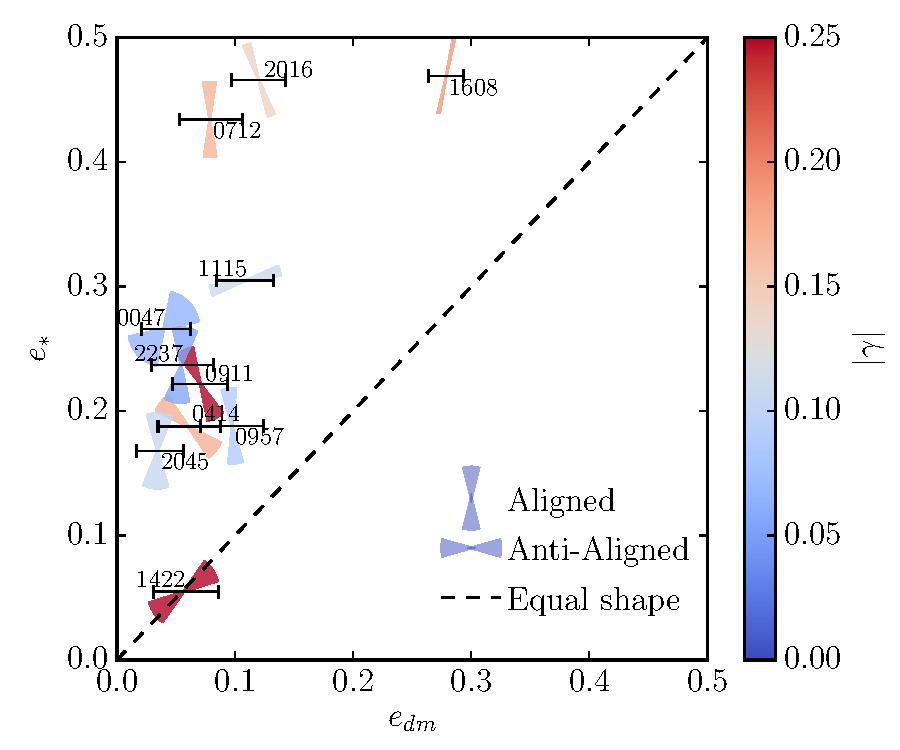
\includegraphics[width=\linewidth]{Figures/wedges_shears.pdf}
  \caption[width=.65\linewidth]{}
  \label{fig:wedges}
\end{figure}

\begin{figure*}
  \centering
  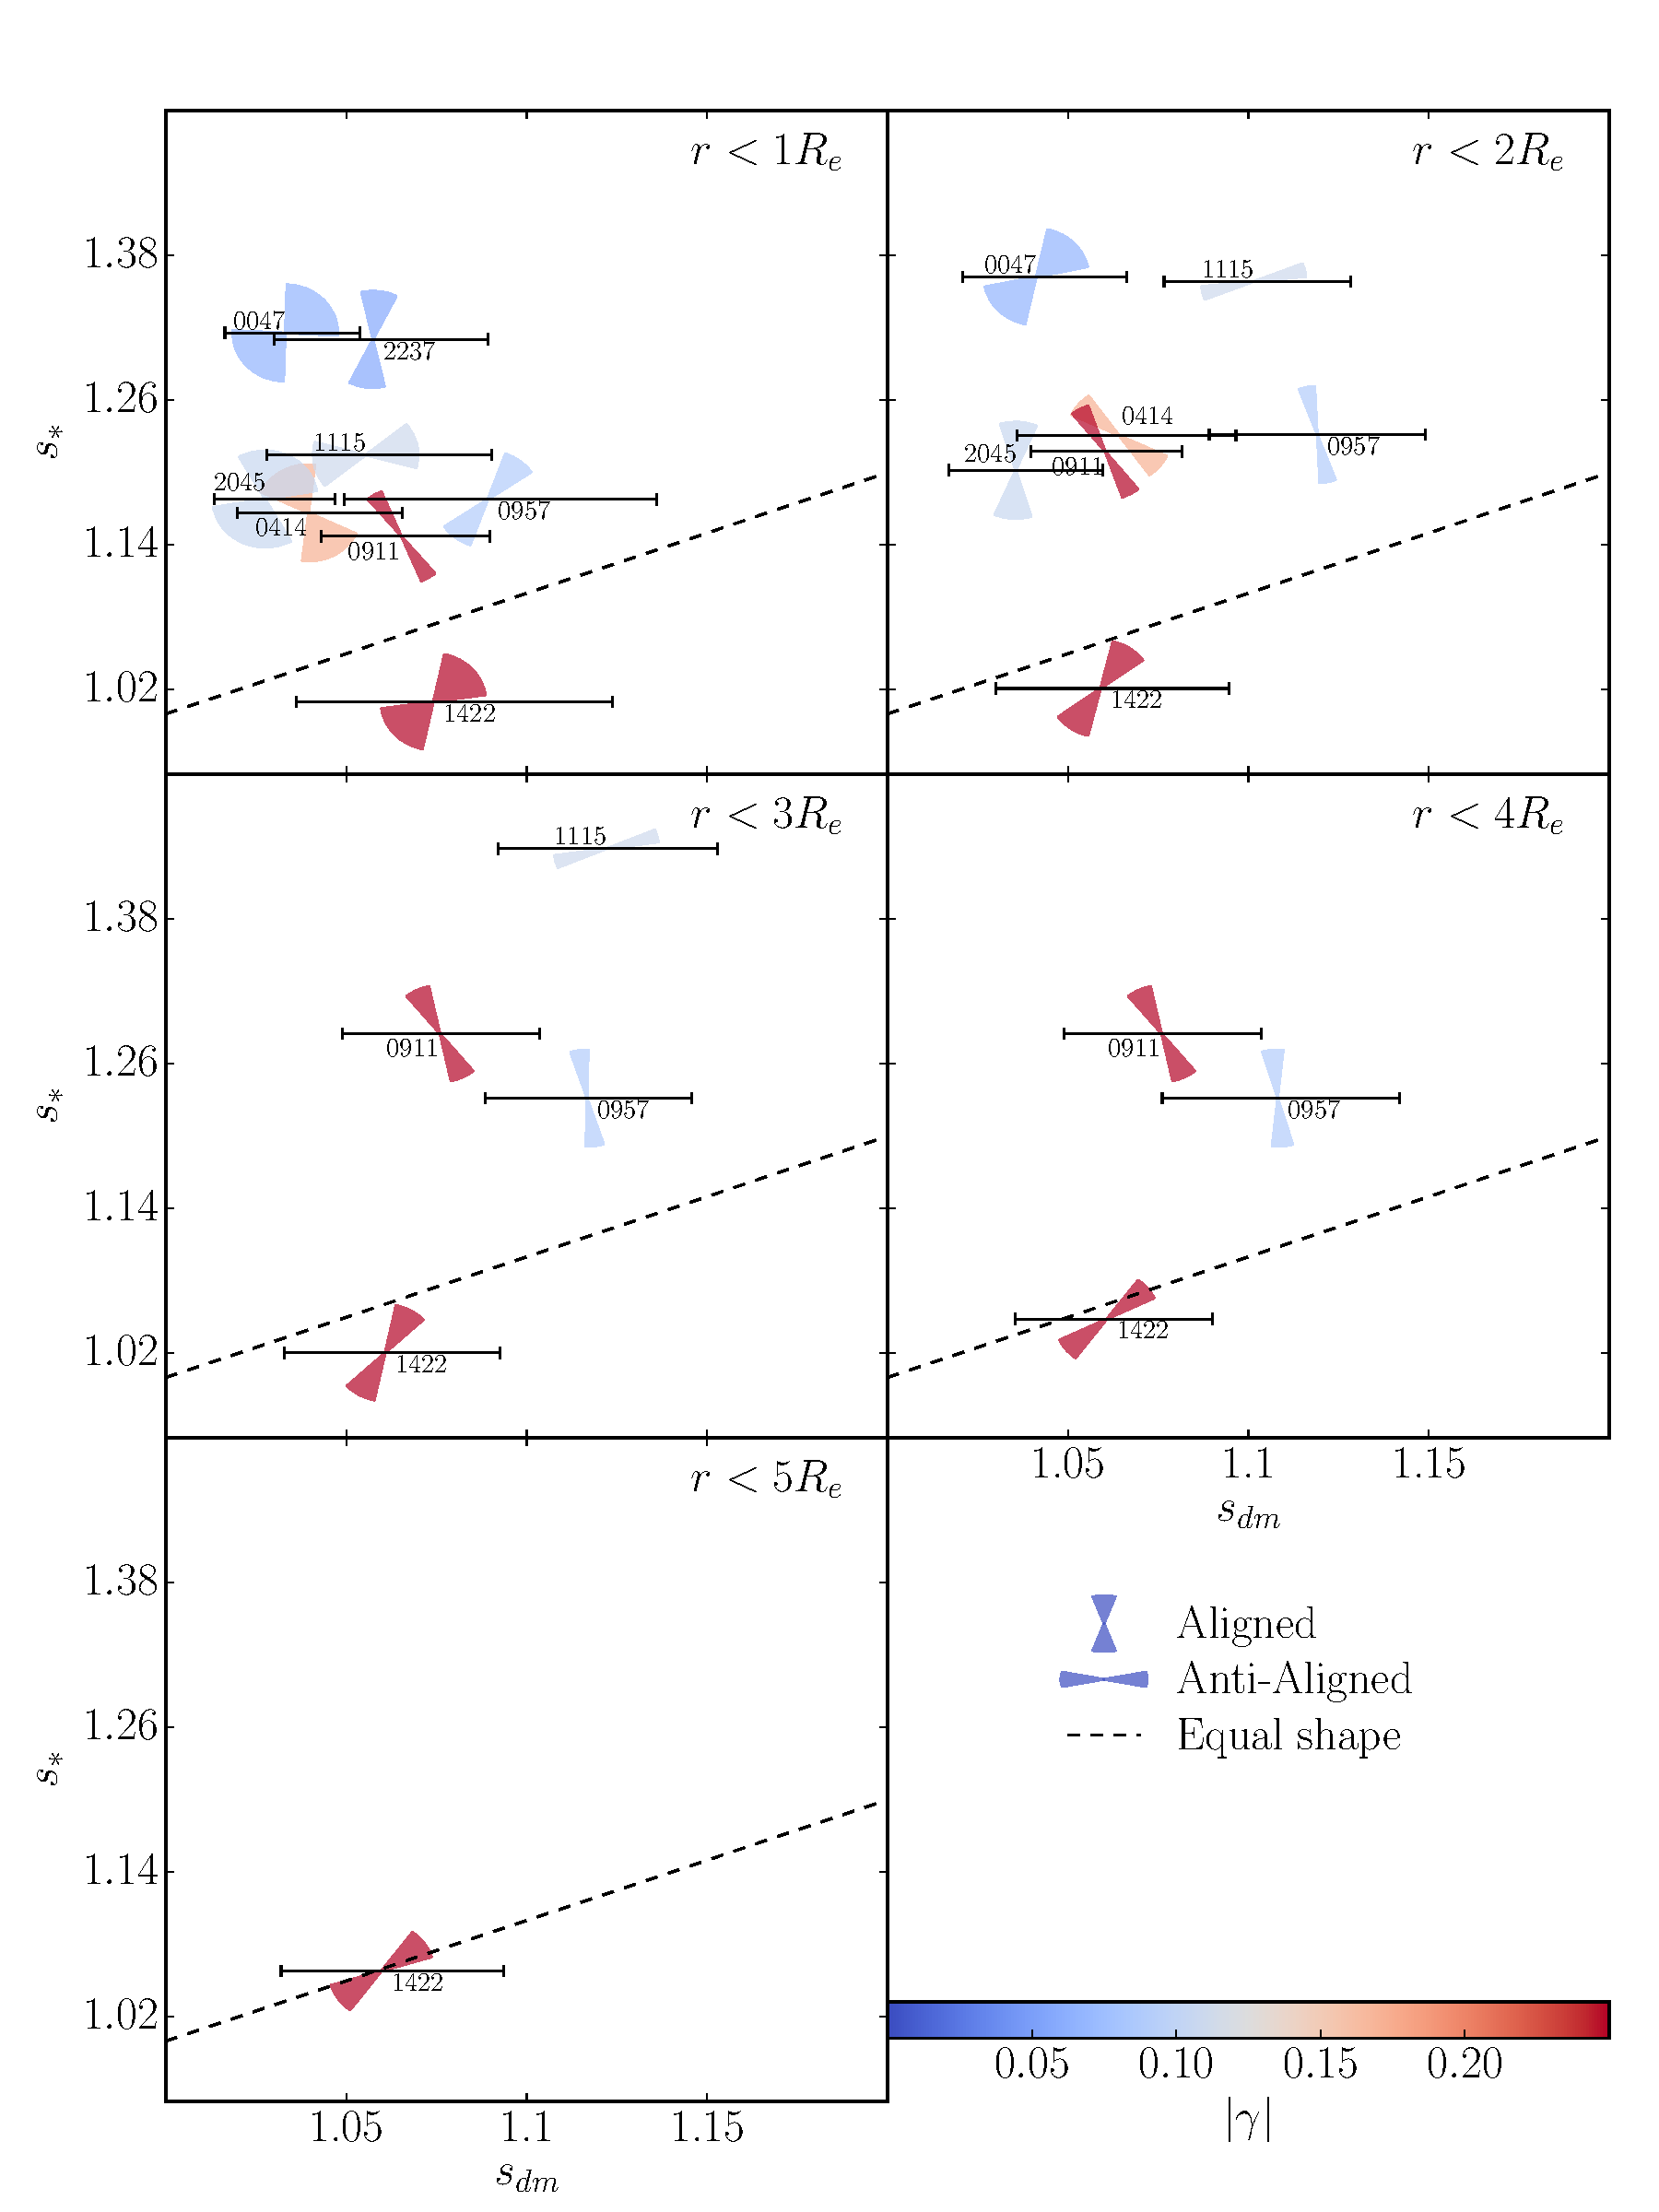
\includegraphics[width=.8\linewidth]{Figures/wedges.pdf}
  \caption[width=.65\linewidth]{}
  \label{fig:wedgesall}
\end{figure*}

\section{Conclusion}\label{sec:conclusions}

{\bf JR. JUSTIN TO WRITE DISCUSSION/CONCLUSIONS ONCE FINAL PLOTS ARE FINISHED.} 


\section{Acknowledgements}\label{sec:acknowledgements}
We would like to thank Dominik Leier for useful discussions. JIR would like to acknowledge support from SNF grant PP00P2\_128540/1.

\bibliographystyle{mn2e}
\bibliography{paper}

\appendix
\section{Reconstructed Lenses}\label{sec:reconstructions}

In this appendix, we show the results of our lens modelling for each individual lens (Figures \ref{fig:lensreconstruction1}, \ref{fig:lensreconstruction2}, and \ref{fig:lensreconstruction3}). The panels show, from left to right: the arrival time surface; the surface mass density of the dark matter; and the surface mass density of the stars. The solid lines mark the eigenvalues and eigenvectors of the 2D moment of inertia tensor in each case; the dotted lines the 68\% confidence interval of these for the dark matter map. Figure \ref{fig:wedges} is constructed from the ratio of largest to smallest eigenvalue in each case (to measure the shape parameter $s$), and the angle between the dark matter and stellar major axes. Note that the angular scale is always the same for the dark matter and stellar maps, but varies between the different lenses as marked on the Figure axes. 

\begin{figure*}
  \centering
  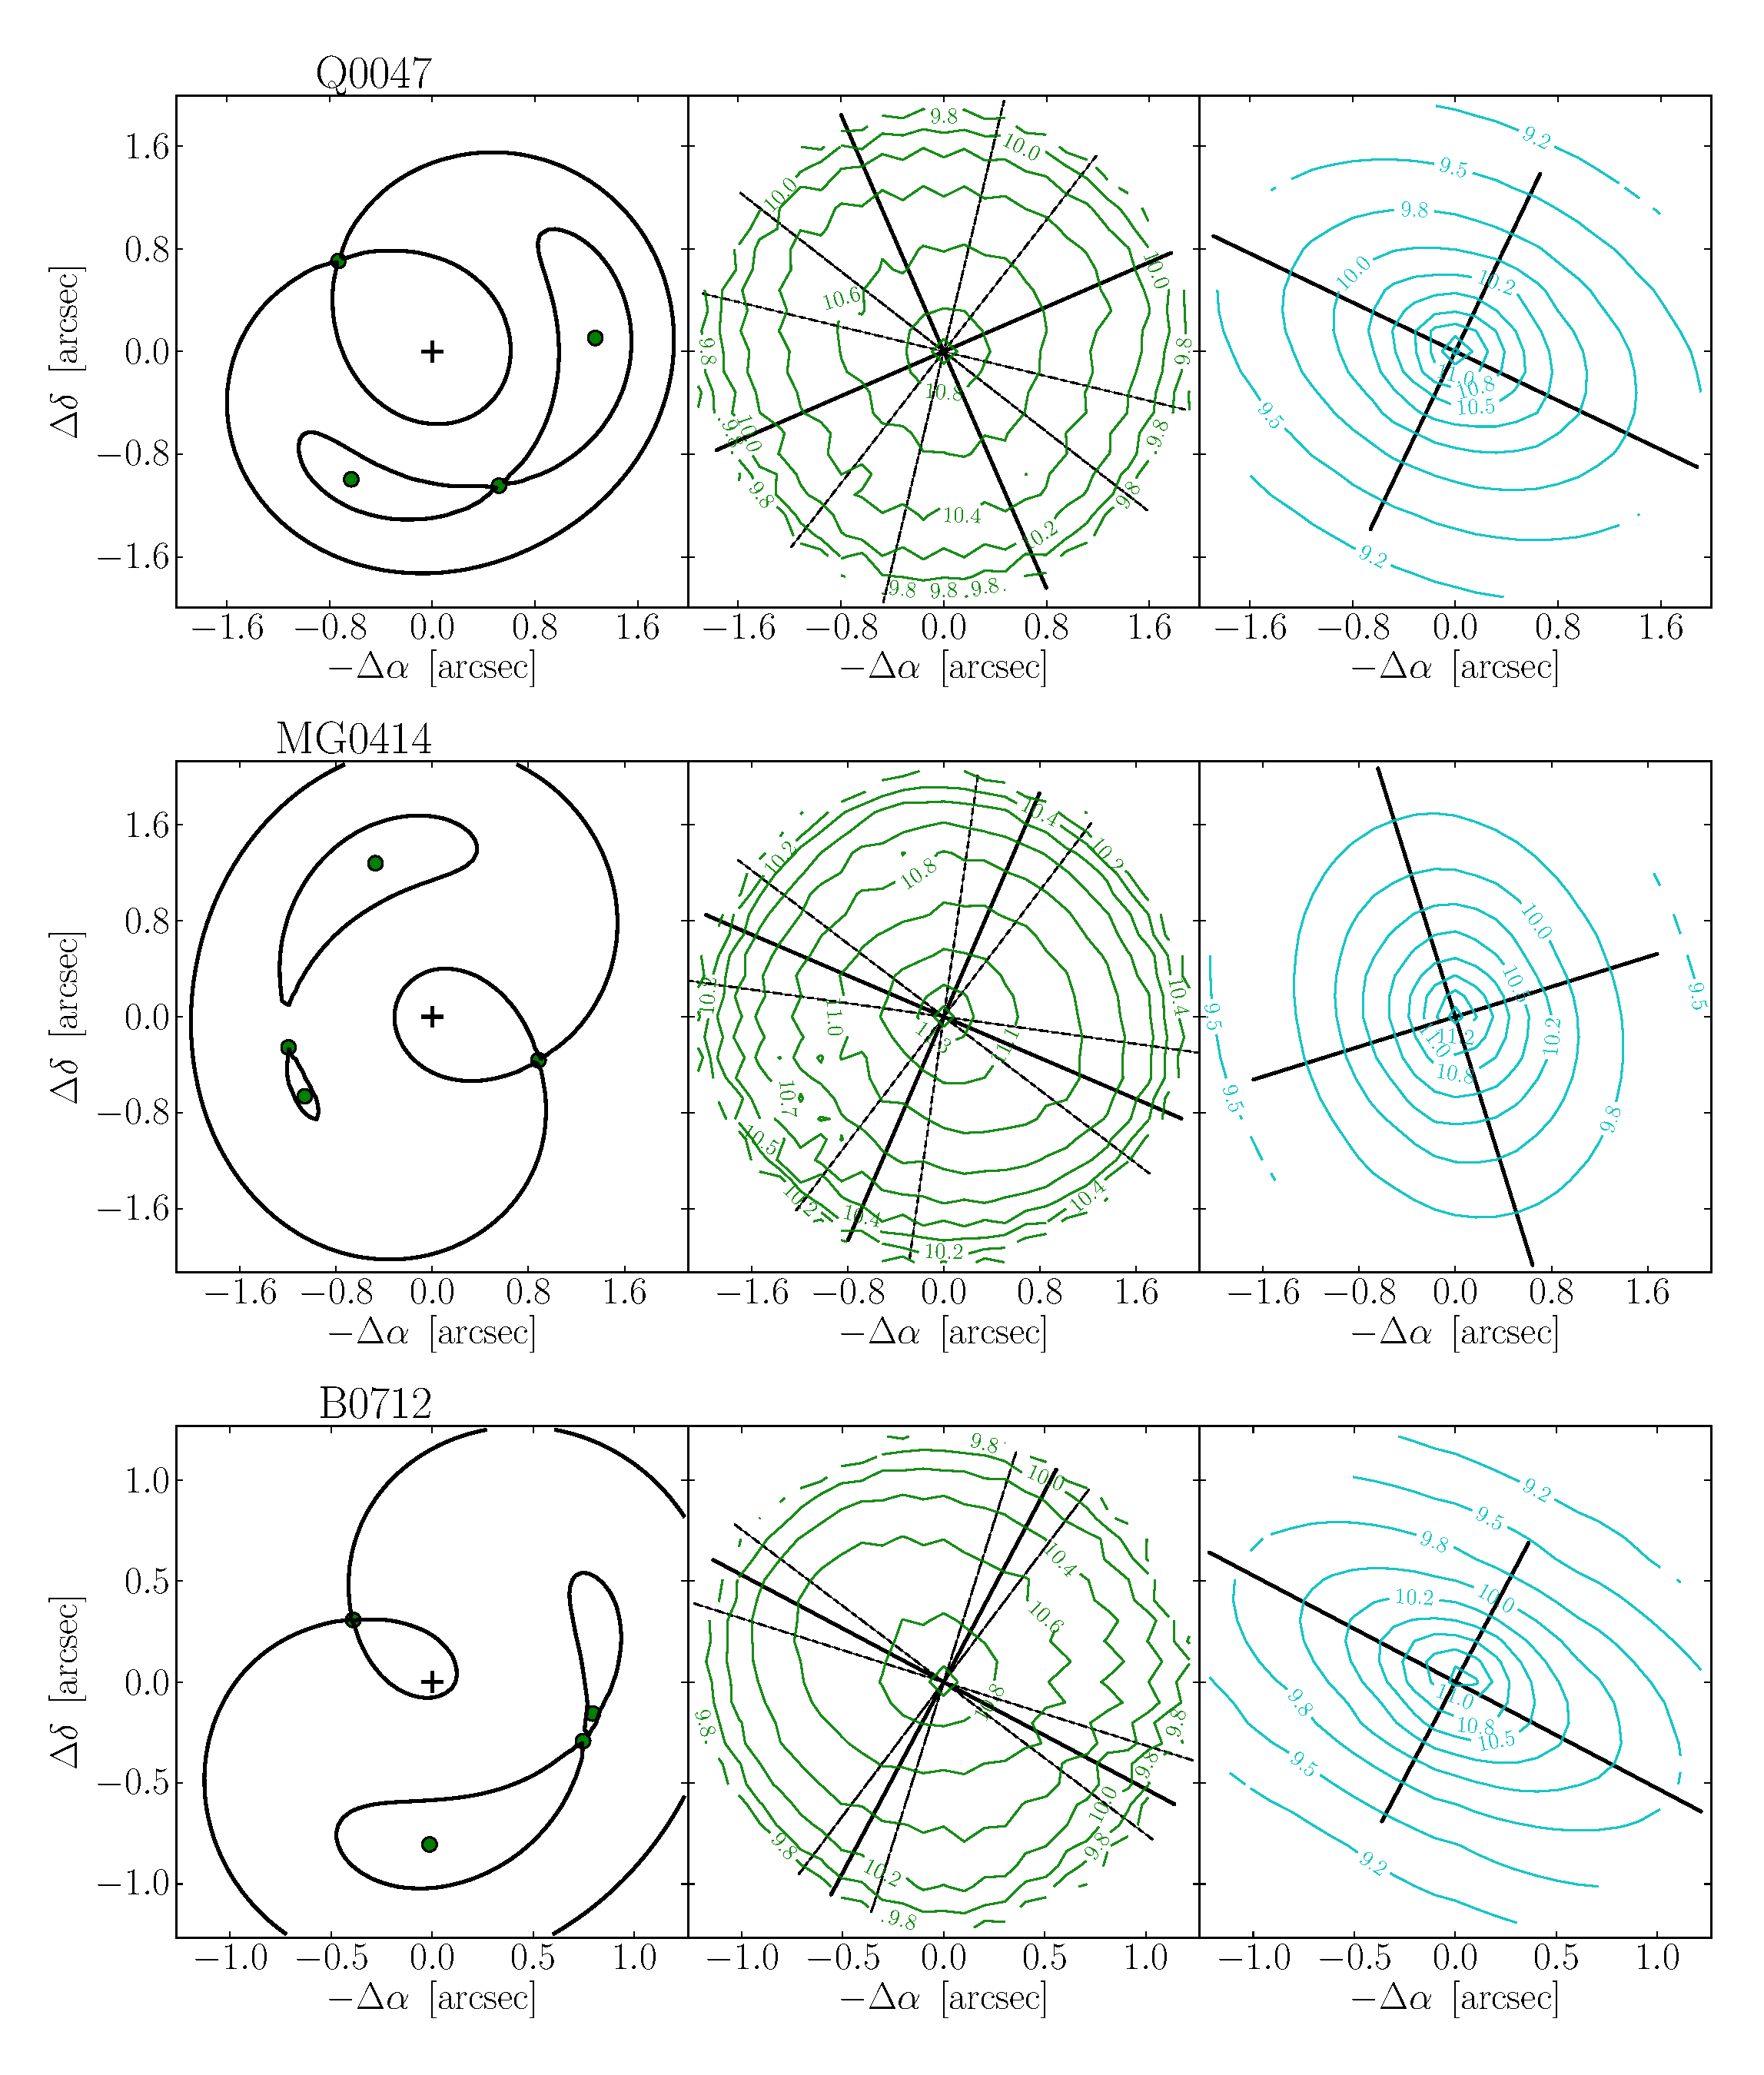
\includegraphics[width=.8\linewidth]{Figures/AllLenses31.pdf}
  \caption[width=.65\linewidth]{The results of our lens modelling for each individual lens. The panels show, from left to right: the arrival time surface (the images are marked by the green circles); the surface mass density of the dark matter; and the surface mass density of the stars. The solid lines mark the eigenvalues and eigenvectors of the 2D moment of inertia tensor in each case; the dotted lines the 68\% confidence interval of these for the dark matter map.}
  \label{fig:lensreconstruction1}
\end{figure*}

\begin{figure*}
  \centering
  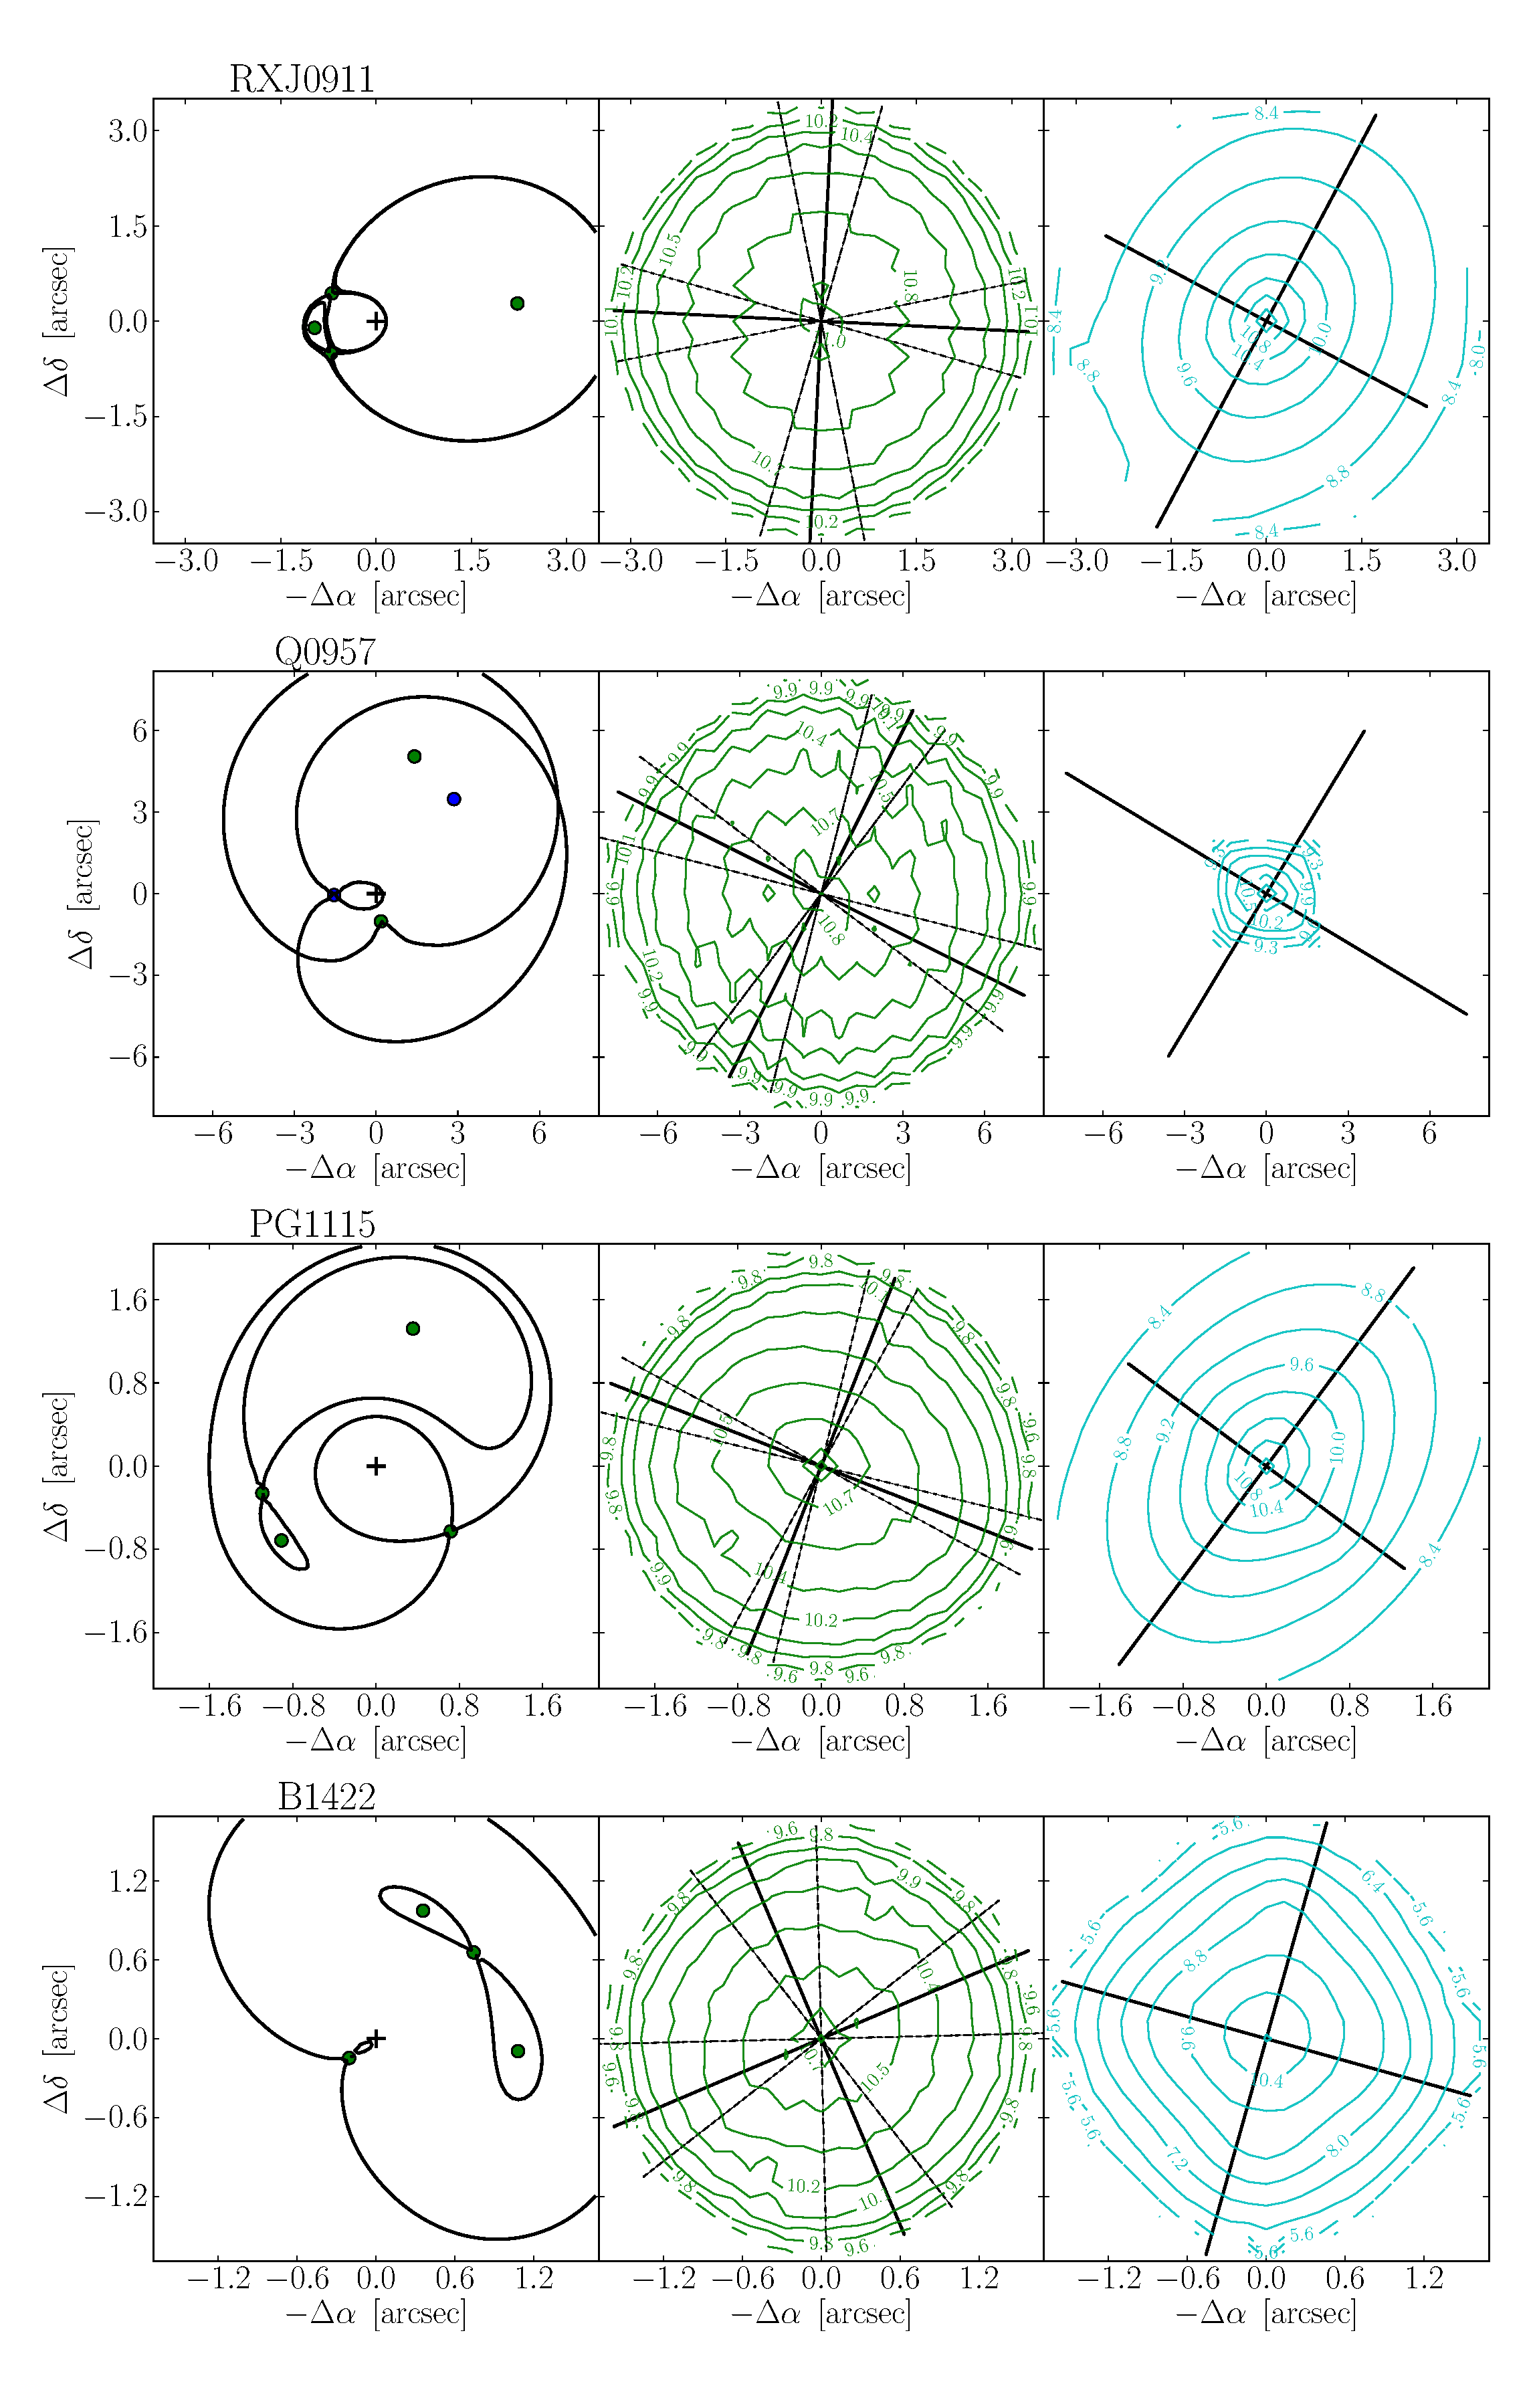
\includegraphics[width=.8\linewidth]{Figures/AllLenses32.pdf}
  \caption[width=.65\linewidth]{The results of our lens modelling for each individual lens. Lines and symbols are as in Figure \ref{fig:ensreconstruction1}.}
  \label{fig:lensreconstruction2}
\end{figure*}

\begin{figure*}
  \centering
  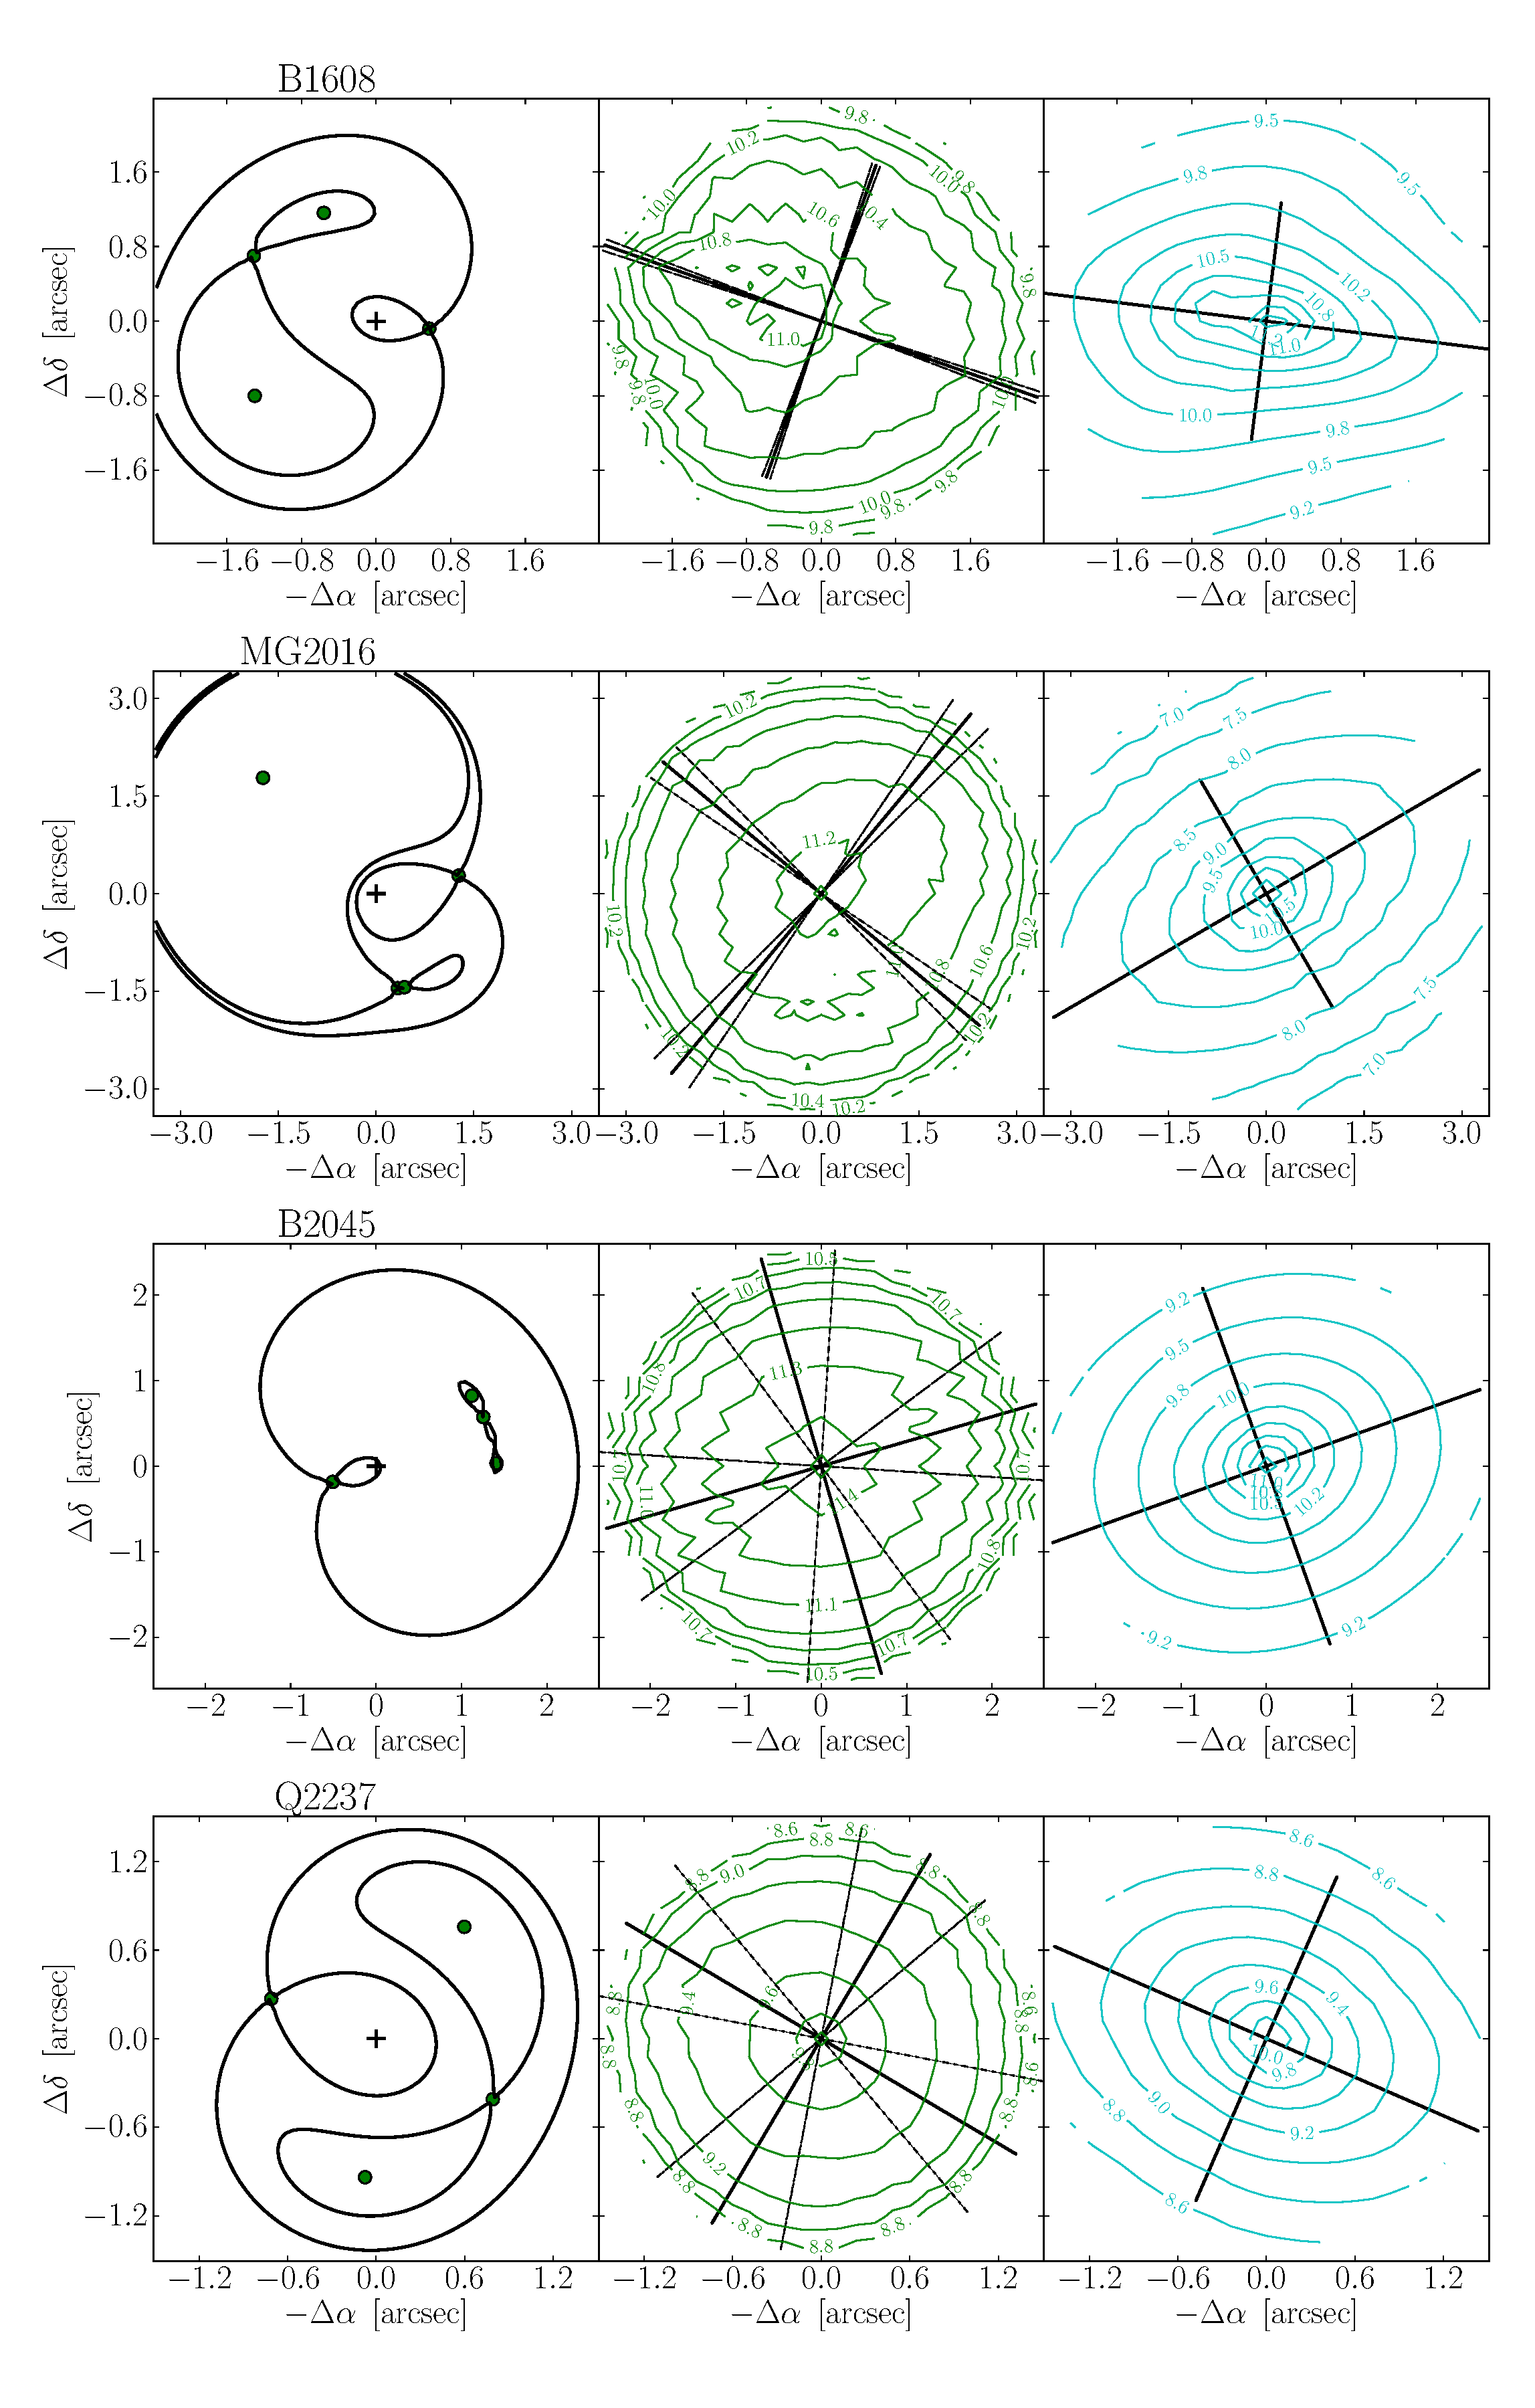
\includegraphics[width=.8\linewidth]{Figures/AllLenses33.pdf}
  \caption[width=.65\linewidth]{The results of our lens modelling for each individual lens. Lines and symbols are as in Figure \ref{fig:ensreconstruction1}.}
  \label{fig:lensreconstruction3}
\end{figure*}

\end{document}